

\section{Method}
\label{sec:method}

\subsection{Preliminaries}
\textbf{Meta learning:} Aims to develop a learning paradigm capable of acquiring knowledge that generalizes across a variety of (possibly new) tasks (see Fig.~\ref{fig:method_overview} for an overview). This concept of 
``{\it learning to learn}'' can be formally characterized as follows:
\begin{equation}
\min_{\omega} 	
\mathbb{E}_{ \tau \sim p({\cal T})}\;%{{\cal T}_{\tau}\sim p({\cal T})}\; 
{\cal L}( D_{\tau};\omega),
\label{eq:meta}
\end{equation}
where $\tau$ %${\cal T}_{\tau}$ 
denotes the $\tau$-th task sampled from $p(\cal T)$, 
$D_\tau$ represents that dataset of task ${\tau}$, and
%${\cal L}(D;\omega)$ 
${\cal L}(D_{\tau};\omega)$
measures the model performance trained  with $\omega$ on the dataset $D_{\tau}$. In ~\cref{eq:meta}, $\omega$ is known as {\it meta} or {\it across-task} knowledge~\cite{hospedales2021meta}. 
%Solving ~\cref{eq:meta} requires to assume access to a set of source tasks, i.e.  in $D_s$, sampled from $p({\cal T})$, using  {\it support} (training $D_{S}^{\rm tr}$) and {\it query} (validation $D_{S}^{\rm val}$) sets that are used in the meta training as follows:
Solving~\cref{eq:meta} assumes access to source tasks sampled from $p(\mathcal{T})$. Each task is associated with its own dataset $D_s$,  partitioned into a \emph{support} (training) set $D_{S}^{\rm tr}$ and a \emph{query} (validation) set $D_{S}^{\rm val}$  that are used in the meta training:
\begin{equation}
    \omega^{\star} =  \arg\max_{\omega}  \log p(\omega| D_S).
    \label{eq:meta_training_0}
\end{equation}
%As shown later in Sec.~\ref{sec:Meta}, Eq.~\ref{eq:meta_training_0} is solved using a bi-level optimization approach.

\textbf{SpiderMark:}
SpiderMark is an in-generation diffusion watermarking framework that blends a fixed spider-web pattern into the Fourier representation of the initial latent noise.
At verification time, it reconstructs an estimate of the initial latent from a query image and uses a learned frequency-domain verifier, optionally augmented with PSNR and $\ell_1$ similarity cues, to predict watermark presence.
We keep the watermark pattern, diffusion generator, inversion procedure, and verifier architecture unchanged and modify only how the verifier is trained.


\subsection{Problem Setup}



Let $\mathcal{G}$ denote a pretrained diffusion generator and let $W$ be the fixed SpiderMark frequency-domain watermark pattern.
For a prompt $p$ and initial latent noise $x_T$, SpiderMark generates a clean image from $x_T$ and a watermarked image from a modified latent whose Fourier representation is blended with $W$.
We keep this injection procedure unchanged.
Our contribution is the agentic verifier-training procedure: the verifier receives a recovered frequency-domain representation of a query image, optionally together with auxiliary similarity cues, while an agentic scheduler controls which downstream attack tasks are sampled during meta-training.

We assume a set of downstream attack tasks
\begin{equation}
    \mathcal{T} = \{ \tau_1, \ldots, \tau_K \},
\end{equation}
where each $\tau_k$ is an image transformation such as JPEG compression, blur, random crop, occlusion, geometric warp, or a compound augmentation.
Each task preserves the binary verification label but changes the evidence available to the verifier.
An episode for task $\tau_k$ consists of a support set $\mathcal{S}_k$ and a query set $\mathcal{Q}_k$ sampled after applying the same attack transformation.
The goal is to learn verifier parameters $\theta$ that adapt from $\mathcal{S}_k$ and generalize to $\mathcal{Q}_k$, while also learning a task-exposure policy that emphasizes attacks where the verifier currently needs more robust adaptation.

\begin{figure*}[t]
    \centering
    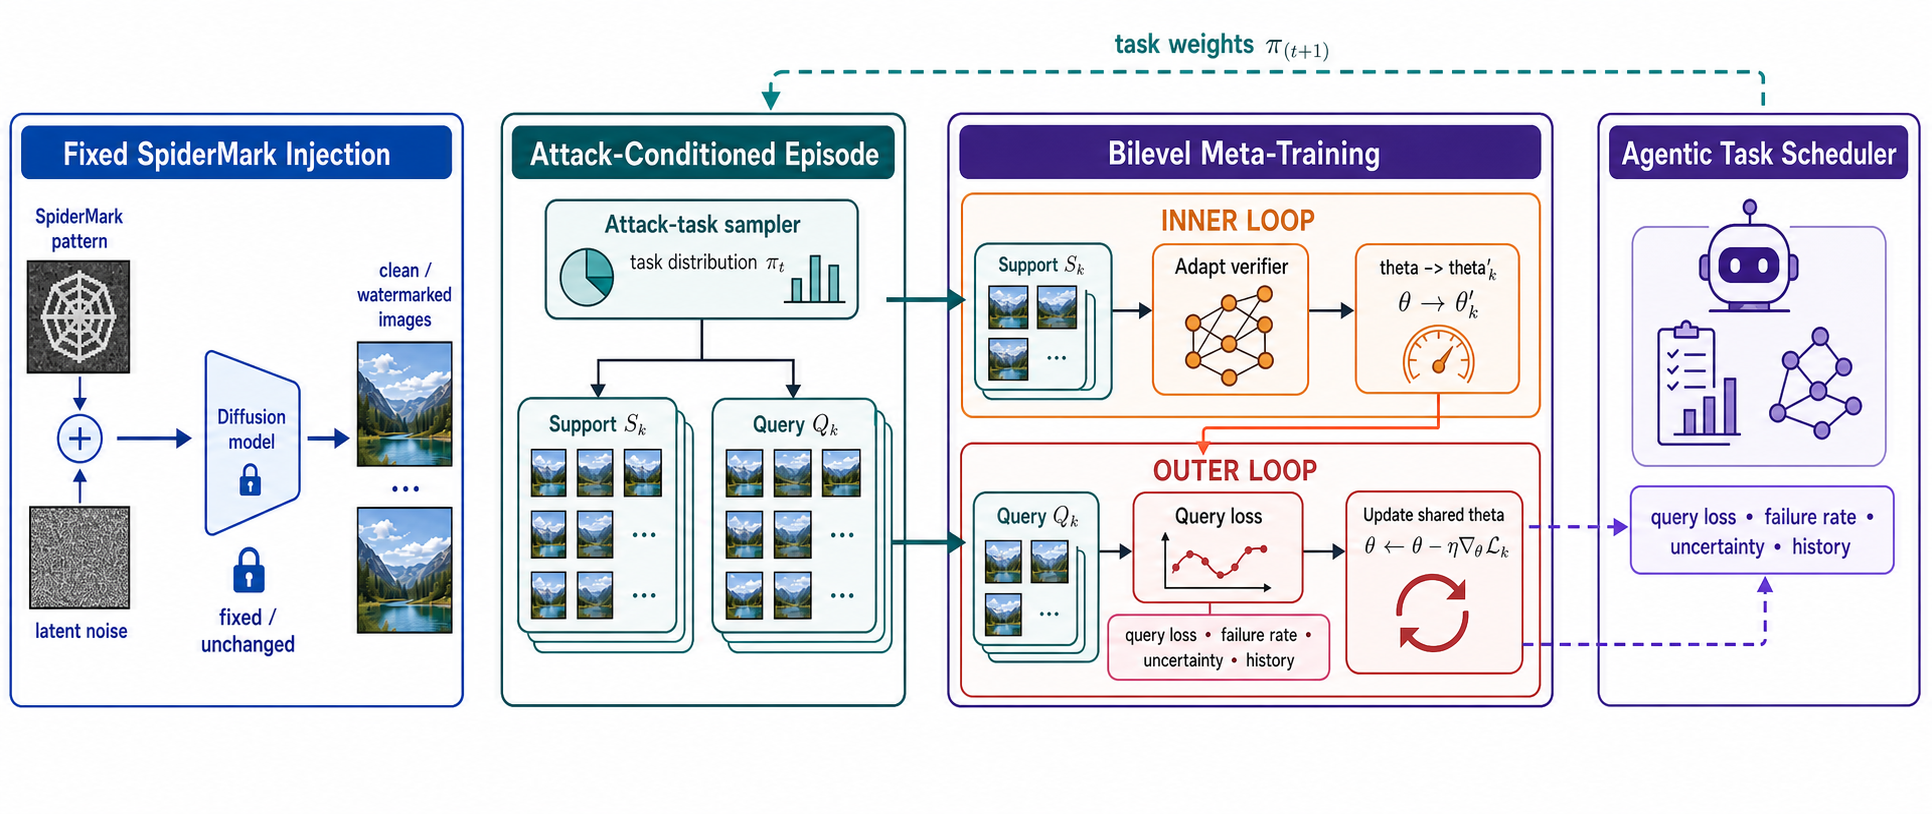
\includegraphics[width=\textwidth]{figures/metaspidermark_overview_inner_outer_imagegen.png}
    \caption{\textbf{Agentic MetaSpiderMark overview.}
    The fixed SpiderMark injection pipeline produces clean and watermarked images without modifying the diffusion generator.
    A task sampler constructs attack-conditioned support and query sets.
    In the inner loop, support examples adapt the shared verifier parameters from $\theta$ to $\theta'_k$; in the outer loop, query loss evaluated at $\theta'_k$ updates the shared initialization $\theta$.
    Query loss, failure rate, uncertainty, and sampling history provide a separate feedback path to the agentic scheduler, whose bounded task weights control subsequent attack sampling rather than watermark injection.}
    \label{fig:method_overview}
\end{figure*}

\subsection{Meta-Compatible Verifier}

The base SpiderMark verifier uses a ResNet-style backbone over frequency-domain inputs and optionally fuses PSNR and $\ell_1$ cues in the final prediction head.
For meta-learning, we implement the verifier using meta-parameterized convolution, batch-normalization, and linear layers.
This allows temporary inner-loop parameter updates without overwriting the base parameters.
Given input spectrum $x$, PSNR cue $s$, and $\ell_1$ cue $d$, the verifier produces logits
\begin{equation}
    f_{\theta}(x, s, d) \in \mathbb{R}^2.
\end{equation}
When auxiliary cues are disabled, the head receives only the learned feature embedding; otherwise it concatenates the backbone feature with $(s,d)$ before classification.
This design preserves the original SpiderMark verifier interface while making its parameters compatible with differentiable inner-loop adaptation.

\subsection{Attack-Conditioned Meta-Training}

For each meta-training iteration $t$, a scheduler samples an attack task $\tau_k$ from a distribution $\pi_t(\tau)$ over $\mathcal{T}$.
We then construct a support set $\mathcal{S}_k$ and query set $\mathcal{Q}_k$ from the SpiderMark verifier dataset.
The dataset wrapper temporarily applies the task-specific augmentation while sampling both sets, then restores the base dataset state.
This keeps each episode attack-conditioned while preserving the same clean/watermarked label space.

Let $\ell(f_{\theta}(z), y)$ be the cross-entropy loss for example $z$ with binary label $y$.
The support and query losses are
\begin{equation}
\begin{aligned}
    \mathcal{L}_{\mathcal{S}_k}(\theta)
    &=
    \frac{1}{|\mathcal{S}_k|}
    \sum_{(z,y)\in\mathcal{S}_k}
    \ell(f_{\theta}(z), y), \\
    \mathcal{L}_{\mathcal{Q}_k}(\theta)
    &=
    \frac{1}{|\mathcal{Q}_k|}
    \sum_{(z,y)\in\mathcal{Q}_k}
    \ell(f_{\theta}(z), y).
\end{aligned}
\end{equation}
The inner update adapts a copy of the verifier parameters using the support loss:
\begin{equation}
    \theta'_k = \theta - \alpha \nabla_{\theta}
    \mathcal{L}_{\mathcal{S}_k}(\theta),
\end{equation}
where $\alpha$ is the inner-loop learning rate.
The outer update optimizes the original parameters using query loss after adaptation:
\begin{equation}
    \min_{\theta}
    \mathbb{E}_{\tau_k \sim \pi_t}
    \left[
    \mathcal{L}_{\mathcal{Q}_k}(\theta'_k)
    \right].
\end{equation}
In the current implementation, the verifier update uses a first-order approximation for efficiency: the query gradient updates the base parameters through the adapted weights while omitting second-order Hessian terms.

\subsection{Agentic Task Scheduler}

The central component of Agentic MetaSpiderMark is the scheduler that controls $\pi_t$.
At iteration $t$, the training loop maintains a compact state summary $h_t$ for each attack task, including usage count, recent query loss, loss change, uncertainty, reward, failure rate, and recency.
This summary is serialized as a structured prompt to an agentic AI controller.
The controller returns a residual scheduling action
\begin{equation}
    a_t = \Delta_t \in \mathbb{R}^{K},
\end{equation}
where each element proposes how much to increase or decrease the sampling weight of one attack task.
To keep the scheduler stable and auditable, the action is not applied directly.
We clip the residual to a bounded range and combine it with a base distribution:
\begin{equation}
    \pi_{t+1}
    =
    \mathrm{normalize}
    \left(
    \pi_{\mathrm{base}} + \lambda \, \mathrm{clip}_{\rho_t}(\Delta_t)
    \right),
\end{equation}
where $\lambda$ controls the maximum scheduler influence and $\rho_t$ is the residual budget at training step $t$.
The local training code therefore retains final authority over valid task probabilities, while the agent supplies adaptive corrections based on online training behavior.

The agentic scheduler differs from non-contextual bandits and hand-designed curricula in two ways.
First, it reasons over a structured multi-signal task state rather than a single scalar reward.
Second, its output is a residual correction, so it can emphasize difficult or under-explored attacks without collapsing coverage of the remaining task pool.
This makes the method model-agnostic: it does not require changing the diffusion generator, watermark pattern, or verifier architecture, and only controls the sequence of attack-conditioned verifier episodes.

\paragraph{Agent protocol and safeguards.}
The scheduler-agent interface is deliberately narrow.
At an agent update step, the training loop sends a JSON state containing the global meta-training context and one row per attack task.
Each task row includes the task name, current base weight, usage count, last sampled step, exponential moving averages of query loss, failure rate, reward, and uncertainty, plus recent-window summaries such as recent loss mean, loss standard deviation, and reward mean.
The global context records training-level signals such as recent meta-loss trend, gradient norm, learning rate, and recent task counts.
The agent is instructed to return only a JSON object with two fields:
\begin{equation}
    \{\texttt{delta\_weights}: [\Delta_1,\ldots,\Delta_K],
    \texttt{rationale}: r\}.
\end{equation}
The response is validated against a fixed JSON schema, and the length of \texttt{delta\_weights} must match the number of attack tasks.
If parsing fails, the API times out, the schema is invalid, or the vector has the wrong shape, the controller falls back to the cached previous residual or the local base scheduler, depending on the run configuration.

The agent never directly sets the sampling distribution.
Every returned residual is clipped to the configured range $[-\rho_t,\rho_t]$, combined with the base policy, lower-bounded by a minimum task weight, and normalized locally.
In the 2000-step agentic run, we start with a conservative residual budget of $\rho_t=0.15$ and switch to $\rho_t=0.5$ at meta-training step 400.
This progressive budget lets the agent first explore with small corrections and then, once task statistics become reliable, make stronger decisions about which attack types should be suppressed because they are saturated, over-sampled, or no longer yielding useful progress.
The default agent call interval is 100 meta-training steps and the recent statistics window is 20 observations.
All agent responses, rationales, cached residuals, API errors, call counts, and latency statistics are logged to the scheduler trace.
This design makes the agentic component reproducible and auditable: the language model proposes bounded residual corrections, while deterministic local code enforces validity, coverage, and probability normalization.

\begin{algorithm}[t]
\caption{Agentic MetaSpiderMark Training}
\label{alg:metaspidermark}
\begin{algorithmic}[1]
\Require SpiderMark verifier dataset $\mathcal{D}$; attack tasks $\mathcal{T}$; verifier $f_\theta$; agentic scheduler $A$; residual-budget schedule $\rho_t$; support size $n_s$; query size $n_q$
\State Initialize base task distribution $\pi_0$ and task statistics $h_0$
\For{each meta-training iteration}
    \State Build task distribution $\pi_t(\tau \mid h_t)$
    \State Sample attack task $\tau_k \sim \pi_t$
    \State Sample support set $\mathcal{S}_k$ and query set $\mathcal{Q}_k$ under $\tau_k$
    \State Copy verifier parameters $\theta$ to task parameters $\theta'_k$
    \State Adapt $\theta'_k \leftarrow \theta'_k - \alpha\nabla_{\theta'_k}\mathcal{L}_{\mathcal{S}_k}(\theta'_k)$
    \State Compute query loss $q_k = \mathcal{L}_{\mathcal{Q}_k}(\theta'_k)$
    \State Update base parameters $\theta \leftarrow \theta - \beta\nabla_{\theta}q_k$
    \State Update task statistics $h_{t+1}$ with $(\tau_k, q_k)$
    \If{agent update interval is reached}
        \State Ask agent $A$ for residual task correction $\Delta_t$ from $h_{t+1}$
        \State Update $\pi_{t+1} \leftarrow \mathrm{normalize}(\pi_{\mathrm{base}} + \lambda\,\mathrm{clip}_{\rho_t}(\Delta_t))$
    \EndIf
\EndFor
\end{algorithmic}
\end{algorithm}

\subsection{Scheduler Baselines}

The benchmark compares the agentic scheduler against non-agentic task-selection strategies under the same verifier, attack pool, support/query sizes, and training budget.
Uniform sampling serves as a minimal anchor, while cyclic scheduling is reserved for diagnostics.
The main comparison includes non-contextual UCB bandit scheduling~\cite{auer2002finite}, ATS-style adaptive scheduling based on meta-model state~\cite{yao2021ats}, BASS-style contextual bandit scheduling~\cite{ban2023bass}, and Adaptive Sampler-style task sampling based on online diversity, entropy, and difficulty statistics~\cite{wang2024tasksampler}.
Our ATS-style and BASS-style controllers are repository-native approximations that preserve the relevant scheduling principle under the SpiderMark attack-task interface; they should be interpreted as SOTA-inspired task-scheduler baselines rather than official reproductions of the original implementations.
The Adaptive Sampler-style row adapts the recent ASr idea to attack tasks by combining under-sampling and recency as a diversity signal, loss volatility as an entropy-like signal, and normalized recent query loss as a difficulty signal.
We also provide optional appendix proxies for GCP-style exponential task weighting~\cite{liu2020adaptive} and DERTS-style representative task selection~\cite{zhan2024derts}.
These baselines let the final evaluation isolate the benefit of agentic scheduling from the benefit of meta-learning itself.

\paragraph{Meta-learning algorithm context.}
The main benchmark fixes the meta-learning update so that scheduler effects are isolated.
For context, the code also supports several fixed-scheduler meta-learning updates: first-order MAML, second-order MAML~\cite{finn2017maml}, ANIL-style head-only inner adaptation, Reptile-style first-order optimization, a \texttt{matching\_net} attention baseline inspired by Matching Networks~\cite{vinyals2016matching}, a \texttt{proto\_net} metric baseline inspired by Prototypical Networks~\cite{snell2017prototypical}, and an \texttt{r2d2\_ridge} baseline inspired by differentiable closed-form solvers~\cite{bertinetto2019meta}.
The \texttt{matching\_net} variant predicts query labels by soft attention over support embeddings.
The \texttt{proto\_net} variant computes support-set class prototypes in the learned embedding space and uses negative squared Euclidean distances as query logits.
The \texttt{r2d2\_ridge} variant fits a ridge classifier on support embeddings and backpropagates the query loss through the linear solve.
This provides a stronger solver-head family for comparison, but it is not a full MetaOptNet SVM/QP reproduction~\cite{lee2019metaoptnet}.
